\tikzset{
  ->,  % makes the edges directed
  node distance=4cm, % specifies the minimum distance between two nodes.
}
\quad
\begin{center}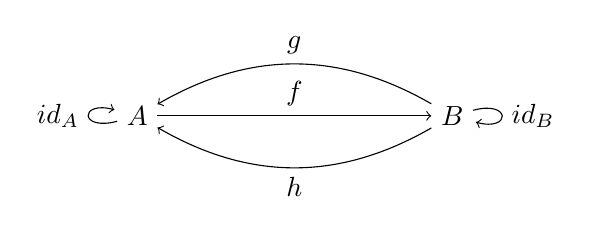
\begin{tikzpicture}
    \node[] (A) {$A$};
    \node[right of=A] (B) {$B$};
    \draw   (A) edge[loop left] node{$id_A$} (A)
            (B) edge[bend right, above] node{$g$} (A)
            (A) edge[above] node{$f$} (B)
            (B) edge[bend left, below] node{$h$} (A)
            (B) edge[loop right] node{$id_B$} (B);
\end{tikzpicture}\end{center}
For arbitrary $f$, let there be two morphs $h$ and $g$ such that $f g = id_B$ and $h f = id_A$. We have $h = h ~ id_A = h (f g) = (h f) g = id_A ~ g = g$, from the definition of the identity map and associativity of the composition operator.